\documentclass[tikz,border=2pt]{standalone}
\usepackage{amsmath,amssymb}
\usepackage{tikz}
\usetikzlibrary{arrows.meta}

\begin{document}
% Polar coordinates: a point is located by its distance r from the origin and the angle theta
% from the positive x-axis; the grid consists of circles and rays.
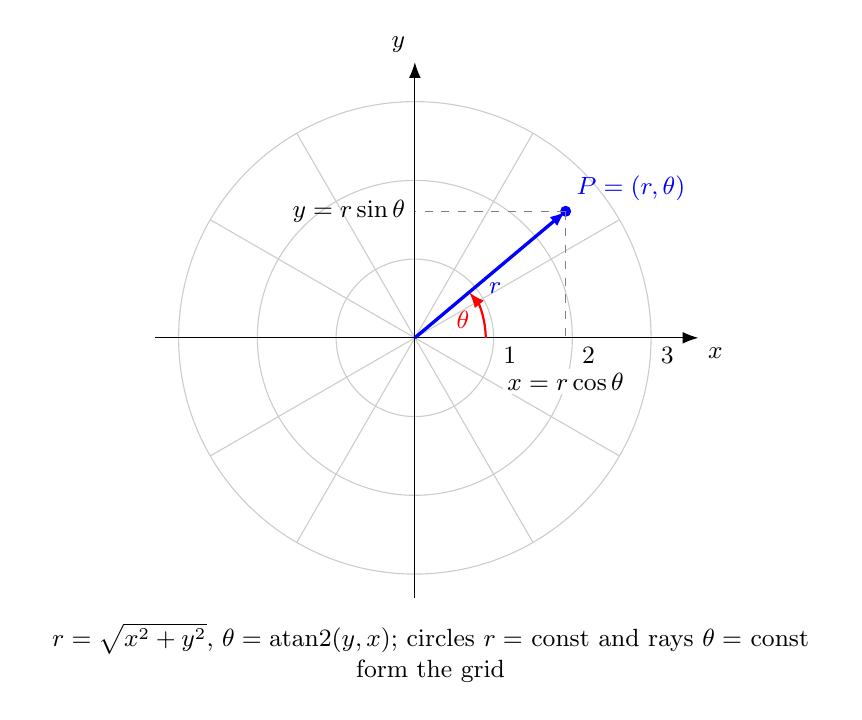
\begin{tikzpicture}[every node/.style={font=\small}, >={Latex[length=2mm]}]
	\foreach \r in {1,2,3} {\draw[gray!40] (0,0) circle (\r);}
	\foreach \a in {0,30,...,330} {\draw[gray!40] (0,0) -- (\a:3);}
	\draw[->] (-3.3,0) -- (3.6,0) node[below right] {$x$};
	\draw[->] (0,-3.3) -- (0,3.5) node[above left] {$y$};
	\foreach \r in {1,2,3} {\node[font=\small, below right] at (\r,0) {$\r$};}
	\draw[->, blue, very thick] (0,0) -- (40:2.5) node[above right] {$P=(r,\theta)$};
	\fill[blue] (40:2.5) circle (2pt);
	\node[blue, above left, font=\small] at (20:1.3) {$r$};
	\draw[red, thick, ->] (0.9,0) arc (0:40:0.9);
	\node[red, font=\small] at (20:0.65) {$\theta$};
	\draw[dashed, gray] (40:2.5) -- ({2.5*cos(40)},0) node[below=11pt, black, font=\small, fill=white, inner sep=1.5pt] {$x=r\cos\theta$};
	\draw[dashed, gray] (40:2.5) -- (0,{2.5*sin(40)}) node[left, black, font=\small] {$y=r\sin\theta$};
	\node[anchor=north, align=flush center, text width=10cm] at (0.2,-3.5) {$r=\sqrt{x^2+y^2}$, $\theta=\operatorname{atan2}(y,x)$; circles $r=$ const and rays $\theta=$ const form the grid};
\end{tikzpicture}
\end{document}
